\documentclass[12pt]{article}
\usepackage[brazil]{babel}
\usepackage{graphicx}
\usepackage{mathtools}
\usepackage{float} 
\usepackage{xcolor}
\usepackage{amsmath, amssymb, bm}


\usepackage{array}
\usepackage{booktabs}



% margenes
\usepackage[a4paper,left=3cm,right=3cm,top=3cm]{geometry}

%opening
\title{}
\author{}

\begin{document}

\begin{center}
	{\tiny {\normalsize {\large \textbf{Convecção}\\ Lista de exercicios 3\\
	
	\textbf{Cristian Herledy Lopez Lara}}}}
\end{center}

\subsection*{Exercício 3,19 livro texto}


\textbf{(a) Mostre que, no diagrama da Figura 1, a vazão de ar através da abertura e a transferência de calor por convecção são dadas pelas expressões}\\

\begin{equation}
	\begin{aligned}
		\dot{m} = (\rho _{q} - \rho _{f}) \frac{g D^{3} HW}{24\nu L} 
	\end{aligned}
\end{equation}

\begin{equation}
	\begin{aligned}
		q = \dot{m} C_{p} (T_{q} - T_{f})
	\end{aligned}
\end{equation}

\begin{figure}[H]
	\centering
	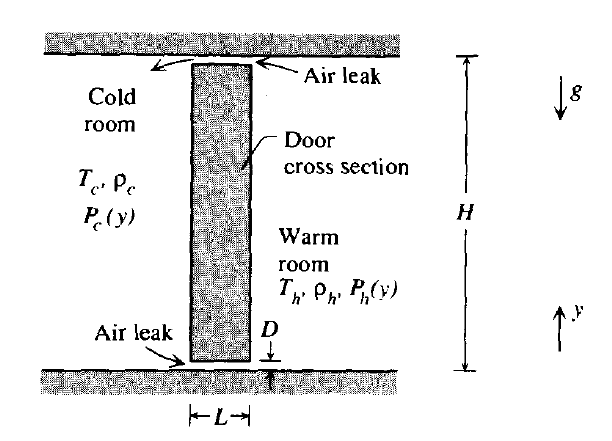
\includegraphics[width=.65\textwidth]{Figures/1_1}
	\caption{Diagrama de fluxo de ar entre volume quente e frio}
\end{figure}


\textbf{Desenvolvimento} 

A pressão em cada volume depende da altura (y). Para cada volume é

\begin{equation}
	\begin{aligned}
		P_{q}(y) = P_{q}(0) - \rho _{q}gy
	\end{aligned}
\end{equation}
\begin{equation}
	\begin{aligned}
		P_{f}(y) = P_{f}(0) - \rho _{f}gy
	\end{aligned}
\end{equation}


\begin{equation}
	\begin{aligned}
		\Delta P(y) = ( \rho _{q} - \rho _{f})g\frac{H}{2}
	\end{aligned}
\end{equation}

Assumindo o fluxo através das aberturas como placas planas, completamente desenvolidas, a velocidade horizontal é calculada usando a equação de Hagen-Poiseuille [1, eq 3.19]. A distribuição de pressão é substituída pela equação (3) y $dx = L$


\begin{equation}
	\begin{aligned}
		U = \frac{D^{2}}{12\mu} \left( \frac{-dP}{dx}\right) 
	\end{aligned}
\end{equation}
\begin{equation}
	\begin{aligned}
		U = \frac{D^{2}}{12\mu} \left( \frac{\rho _{q} - \rho _{f})g\frac{H}{2}}{L}\right) 
	\end{aligned}
\end{equation}

Considerando o fluxo de massa atuando na área $A = WD$ como

\begin{equation}
	\begin{aligned}
		\dot{m} = \rho U WD
	\end{aligned}
\end{equation}

Substituindo U

\begin{equation}
	\begin{aligned}
		\dot{m} = \rho \frac{D^{2}}{12\mu} \left( \frac{(\rho _{q} - \rho _{f})g\frac{H}{2}}{L}\right)  WD
	\end{aligned}
\end{equation}

\begin{equation}
	\begin{aligned}
		\dot{m} = \frac{D^{3}}{24\nu} \frac{(\rho _{q} - \rho _{f})gHW}{L}
	\end{aligned}
\end{equation}

Esta expressão é equivalente à da equação (1)\\

\textbf{(a) Calcular $\dot{m}$ e $q$}\\

Substituindo os valores numéricos em (2) e (10)

\begin{equation}
	\begin{aligned}
		\dot{m} = \frac{{(0,5 x 10^{-3}m^{3})^3} * 0,082 \frac{Kg}{m^{3}}   *  9,81 \frac{m}{s^{2}}  *  2,2m  *  1,5 m  }{24\nu  *  1.52x 10^{-5}\frac{m^{2}}{s}  *   0,05 m} = 1,823 x 10 ^{-5} \frac{Kg}{s}
	\end{aligned}
\end{equation}

\begin{equation}
	\begin{aligned}
		q = 1,823 x 10 ^{-5} \frac{Kg}{s} * 1006 \frac{J}{Kg*K} * 20K = 0,36 W
	\end{aligned}
\end{equation}

A vazão mássica é proporcional à altura da abertura na proporção de $q \sim D^{3}$. Portanto, um aumento em $D$ incrementa diretamente a taxa de transferência de calor. 

\subsection*{Exercício 3,27	 livro texto}
\textbf{Encontrar analiticamente as expressões}\\

\begin{equation}
	\begin{aligned}
		\Delta \widetilde{T}_{min} = \frac{(T_{peak} - T_{0})}{\frac{q''' A}{k_{0}}}
	\end{aligned}
\end{equation}

\begin{equation}
	\begin{aligned}
		\left( \frac{H}{L}\right) _{opt}
	\end{aligned}
\end{equation}

\begin{figure}[H]
	\centering
	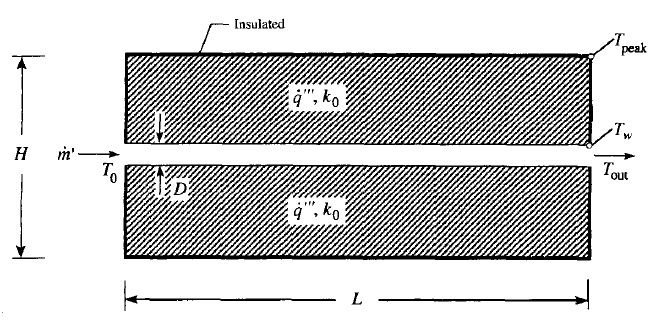
\includegraphics[width=.65\textwidth]{Figures/1_2}
	\caption{Volume sólido 2D com condutividade térmica $k_{0}$}
\end{figure}

\textbf{Desnvolvimento}\\

A área de transferência de calor e, portanto, a área a ser otimizada será dada por $A = HL = cte$. O calor extraído obedece à equação

\begin{equation}
	\begin{aligned}
		Q = q''' HL
	\end{aligned}
\end{equation}

O problema é analisado calculando a queda de temperatura do ponto mais quente $T_{peak}$ até o ponto mais frio $T_{0}$. Na relação $H/L$, o fluxo de calor será perpendicular a U quando $\frac{H}{L} < 1$, y quando $k_{0}$ tem valores baixos.
\\
Assim, a queda de temperatura entre o ponto mais quente $T_{peak}$ e a saída do duto com o ar aquecido $T_{0}$ será dada pela equação de condução deduzida por [2, eq. 4.1]

\begin{equation}
	\frac{\Delta Tk}{q''' A} = \frac{1}{8} \times \frac{H}{L}
\end{equation}

\begin{equation}
	(T_{peak} - T_{w}) = \frac{q'''HA}{8k}
\end{equation}

E o aumento da temperatura por convecção ao longo da direção do fluxo será dado por

\begin{equation}
	(T_{out} - T_{0}) = \frac{q'''HL}{\dot{m} C_{p}}
\end{equation}

O excesso de temperatura é então a soma de ambas as expressões

\begin{equation}
		\Delta \widetilde{T} = (T_{peak} - T_{w}) + (T_{out} - T_{0}) = \frac{q'''HA}{8k} + \frac{q'''HL}{\dot{m} C_{p}}
\end{equation}

Esta equação pode ser adimensional através das seguintes relações

\begin{equation}
	H_{adim} = \frac{H}{\sqrt{A}} \ ,  \ L_{adim} = \frac{L}{\sqrt{A}} \ , \ M = \frac{\dot{m} C_{p} \sqrt{A}}{k}
\end{equation}

\begin{equation}
	\Delta \widetilde{T} = \frac{H_{adim}}{8L_{adim}} + \frac{1}{MH_{adim}}
\end{equation}

O valor ótimo desta expressão é calculado com a derivada igual a zero, considerando $H\sim \frac{1}{L}$.

\begin{equation}
	\Delta \widetilde{T} = \frac{H_{adim}^{2}}{8} + \frac{1}{MH_{adim}}
\end{equation}

\begin{equation}
	\frac{d}{dH_{adim}}\Delta \widetilde{T} = \frac{2H_{adim}}{8} - \frac{1}{MH_{adim}^{2}} = 0
\end{equation}
\begin{equation}
	 \sim \frac{H_{adim}^{3}}{4} - \frac{1}{M} \sim H_{opt} = \left( \frac{M}{4}\right) ^{\frac{1}{3}}
\end{equation}

Como $H\sim \frac{1}{L}$.
\begin{equation}
	L_{opt} = \left( \frac{4}{M}\right) ^{\frac{1}{3}}
\end{equation}

Quais são as expressões equivalentes a (14). É importante concluir que estas relaçãoes de aspecto global $H_{opt}$ e $L_{opt}$ sao independentes de D.  Agora, sustituindo em (21)



\begin{equation}
	\Delta \widetilde{T}_{min} = \frac{\left( \frac{M}{4}\right) ^{\frac{1}{3}}}{8\left( \frac{4}{M}\right) ^{\frac{1}{3}}} + \frac{1}{M\left( \frac{M}{4}\right) ^{\frac{1}{3}}} \sim 0,94 M^{\frac{1}{3}}
\end{equation}

Quando a vazão mássica $\dot{m}$ e a área $A$ são grandes, $M$ aumenta. Com esta suposição, os cálculos serão válidos quando $M > 4$



\begin{equation}
	M = \frac{\dot{m} C_{p} \sqrt{A}}{k} > 4
\end{equation}

Portanto, o fluxo de massa $\dot{m}_{min}$ para garantir $\Delta \widetilde{T}_{min}$ e manter a relação de aspecto ideal $\left( \frac{H}{L}\right)_{opt} $ será

\begin{equation}
	M > \frac{4k}{C_{p}\sqrt{A}}
\end{equation}


\subsection*{Exercício demonstração}
\textbf{Determinar o número de Nusselt para um escoamento interno, laminar, plenamente desenvolvido, com propriedades constantes, seção transversal circular e sujeito a um fluxo de calor uniforme na superfície.}\\

\begin{figure}[H]
	\centering
	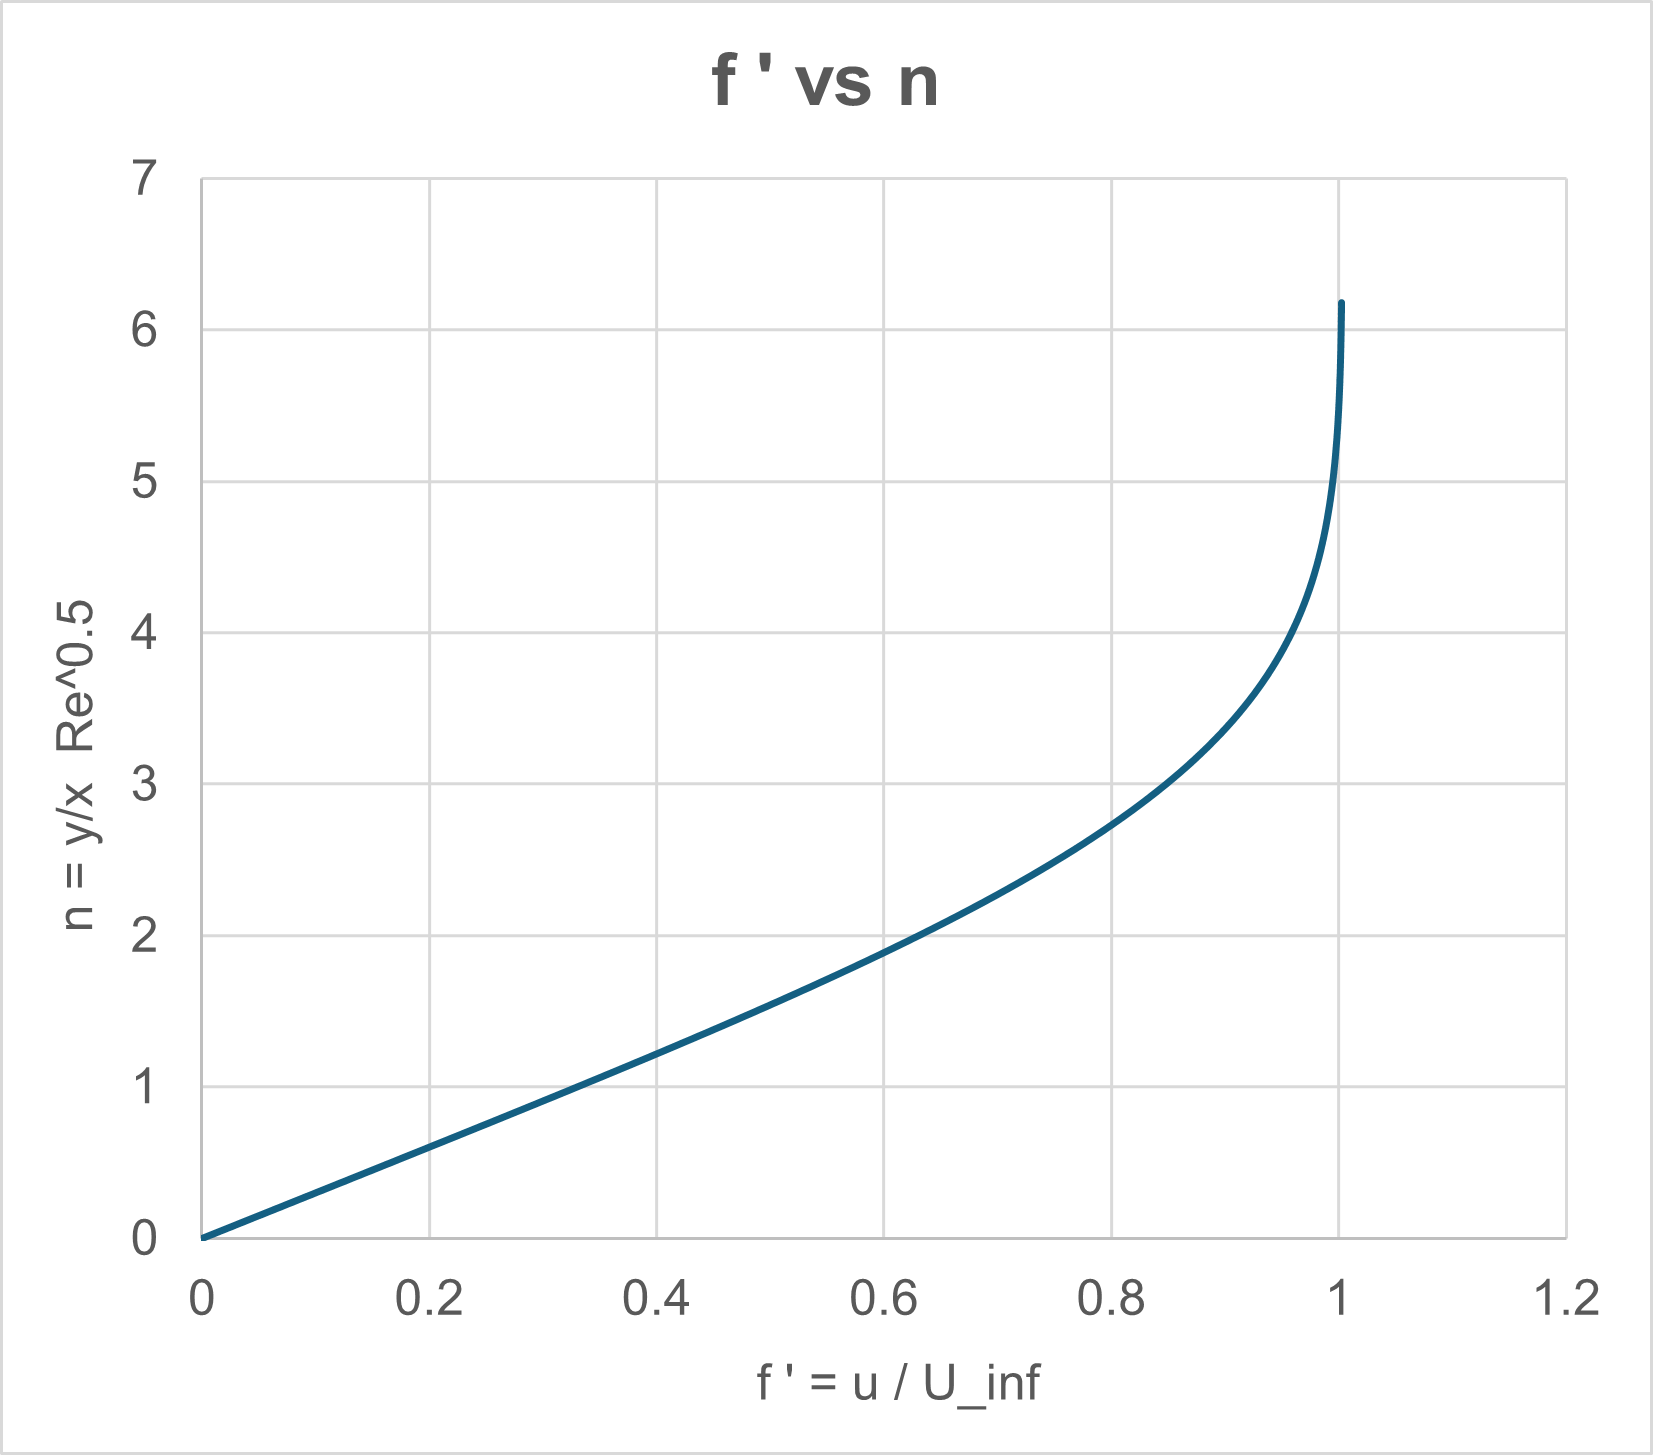
\includegraphics[width=.65\textwidth]{Figures/1_3}
	\caption{Balanço de energia no volume diferencial dentro de um tubo com fluxo de calor uniforme nas paredes}
\end{figure}

Realizando um balanço de energia sem fluxo de calor por conducção como na Figura 3, a equação de energia para o volume diferencial é descrita por

\begin{equation}
	u \frac{\partial T}{\partial x} = \frac{\alpha}{r} \frac{\partial}{\partial r} \left( r \frac{\partial T}{\partial r} \right)
\end{equation}

Reemplazando o gradiente axial da temperatura em termos da temperatura media e superficial, fica

\begin{equation}
	 \frac{\partial T}{\partial x} = \frac{(T_s - T)}{(T_s - T_m)} \frac{d T_m}{d x} 
\end{equation}


\begin{equation}
	\frac{1}{r} \frac{\partial}{\partial r} \left( r \frac{\partial T}{\partial r} \right) = \frac{2 u_m}{\alpha} \left( \frac{d T_m}{d x} \right) \left[ 1 - \left( \frac{r}{r_o} \right)^2 \right]
\end{equation}

Integrando duas vezes para obter o perfil T, obtemos

\begin{equation}
	T(r, x) = \frac{2 u_m}{\alpha} \left( \frac{d T_m}{d x} \right) \left[ \frac{r^2}{4} - \frac{r^4}{16 r_o^2} \right] + C_1 \ln r + C_2 	
\end{equation}
\begin{equation}
	CC1 = T = T_{(x,r)} @ r=0	\ \ CC2 = T_{rmax} = T_{s}(x) @ r=r_{0}
\end{equation}

Aplicando as condições de contorno, $C_{1} = 0$ e $C_{2}$:


\begin{equation}
	C_2 = T_s(x) - \frac{2 u_m}{\alpha} \left( \frac{d T_m}{d x} \right) \left( \frac{3 r_o^2}{16} \right)
\end{equation}

Sustituindo na eq. (32)

\begin{equation}
	T(r, x) = T_s(x) - \frac{2 u_m r_o^2}{\alpha} \left( \frac{d T_m}{d x} \right) \left[ \frac{3}{16} + \frac{1}{16} \left( \frac{r}{r_o} \right)^4 - \frac{1}{4} \left( \frac{r}{r_o} \right)^2 \right]
\end{equation}

Reemplazando as expressões para temperatura media y perfil de velocidade axial
\begin{equation}
	T_m = \frac{2}{u_m r_o^2} \int_0^{r_o} u T r \, dr \ , \ \frac{u(r)}{u_m} = 2 \left[ 1 - \left( \frac{r}{r_o} \right)^2 \right]
\end{equation}

\begin{equation}
	T_m(x) = T_s(x) - \frac{11}{48} \left( \frac{u_m r_o^2}{\alpha} \right) \left( \frac{d T_m}{d x} \right)
\end{equation}
 Usando a equacao do fluxo masico, obtem-se
 \begin{equation}
 	\dot{m} = \rho u_m \left( \pi \frac{D^2}{4} \right)
 \end{equation}
 
 \begin{equation}
 	T_m(x) - T_s(x) = - \frac{11}{48} \frac{q''_s D}{k}
 \end{equation}
 
E com $q''_s = h (T_s - T_m)$
\begin{equation}
	h = \frac{48}{11} \left( \frac{k}{D} \right)
\end{equation}
\begin{equation}
	Nu_D \sim \frac{hD}{k} = 4.36
\end{equation}
A uma taxa de transferência de calor constante

\begin{thebibliography}{999}
	
	\bibitem{abejan}
	Adrian Bejan,
	Convection Heat Transfer.
	Durham, North Carolina,
	3rd Edition,
	2004.
	
	\bibitem{naraghi}
	Adrian Bejan,
	Shape and structure from engineering to nature.
	Cambridge University, USA.
	2000.
	
\end{thebibliography}



\end{document}





